\subsubsection{14.01.15}
\begin{enumerate}
	
	\item Время начала и окончания собрания: 18:10 - 21:00.
	
	\item Цели собрания: 
	\begin{enumerate}
		
		\item Перенести перекладину, неподвижно закрепленную на роботе, чуть выше.
		
	\end{enumerate}

	\item Проделанная работа:
	\begin{enumerate}
		
		\item На соревнованиях в Рязани мы столкнулись с такой проблемой: после того, как нижняя перекладина нижней подвижной рейки слетела с креплений и была перенесена нами чуть выше, подъемник начал очень сильно трястись в процессе раздвигания. Это было связано с тем, что нижняя пара реек не раздвигалась до конца, поскольку нижняя перекладина подвижной рейки при полном раздвигании оказывалась выше верхней неподвижной. Для того, чтобы подъемник двигался плавно, было решено перенести неподвижную перекладину чуть выше таким образом, чтобы нижняя пара реек раздвигалась до конца и не болталась.
        \begin{figure}[H]
	  	  \begin{minipage}[h]{0.2\linewidth}
	  	    \center  
	  	  \end{minipage}
	  	  \begin{minipage}[h]{0.6\linewidth}
	  		\center{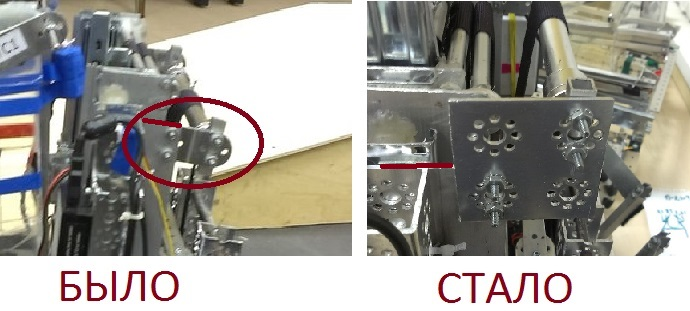
\includegraphics[scale=0.35]{days/14.01.15/images/01}}
	  		\caption{Перекладина перенесена выше}
	  	  \end{minipage}
	   \end{figure}

	\end{enumerate}
	
	\item Итоги собрания:
	\begin{enumerate}
		
		\item Перекладина перенесена выше, но испытания подъемника не проведены.
		
	\end{enumerate}
	
	\item Задачи для последующих собраний:
	\begin{enumerate}
		
		\item Потренироваться в управлении роботом.
		
		\item Провести испытания подъемника.
			
	\end{enumerate}
\end{enumerate}
\fillpage
